% Describe how the experiments are performed

\subsection{Tyrimo metodika}

Visa tyrimo metodika pavaizduota \ref{fig:methodology}-ame pav. Tyrimo tikslas yra nustatyti, ar \LIME ir \gls{mca} metodų sintezė geba efektyviai aptikti \glsplka{adversarial} ir ar šio metodo tikslumas didesnis nei Tcydenovos ir kt. pasiūlyto \LIME pritaikymo \glsplko{adversarial} aptikimui. Tyrimui pasirinktas \SLEIPNIR \cite{al-dujailiAdversarialDeepLearning2018} duomenų rinkinys, kuriame yra $34995$ kenkėjiškų programų ir $19696$ nekenkėjiškų programų pavyzdžių, užkoduotų $22761$-mačiais dvejetainiais vektoriais. Iš šio rinkinio pasirinkta po $1500$ unikalių kenkėjiškų ir nekenkėjiškų programų pavyzdžių paliekant pirmas $200$ komponenčių -- taip gaunamas subalansuotas duomenų rinkinys. Šis rinkinys toliau skeliamas į mokymo ir testavimo aibes santykiu $4:1$. Eksperimentams atlikti paruošiamos šios priemonės:
\begin{enumerate}
    \item Testavimo duomenų aibė.
    \item \textit{MalGAN} \cite{huGeneratingAdversarialMalware2017} \gls{ae} generatorius.
    \item Kenkėjiškų programų detektorius (klasifikatorius).
    \item \Glsplko{adversarial} aptikimo komponentas
    \begin{itemize}
        \item Naudojantis originalius požymius.
        \item Naudojantis \gls{mca} transformuotus požymius \skyrius{sec:method}{}.
    \end{itemize}
\end{enumerate}

Su šiais įrankiais atliekami 3 eksperimentai:
\begin{enumerate}
    \item Bazinis atvejis -- klasifikatoriaus be \glsplko{adversarial} aptikimo metodų tikslumo nustatymas.
    \item Klasifikatoriaus su \LIME metodo pritaikymo \glsplko{adversarial} aptikimui modifikacija tikslumo nustatymas.
    \item Klasifikatoriaus su \LIME ir \gls{mca} metodų sintezės \glsplko{adversarial} aptikimui modifikacija tikslumo nustatymas.
\end{enumerate}


\subsection{\gls{mca} komponenčių pasirinkimas}
Komponenčių pasirinkimas yra \ref{fig:methodology}-ame pav. minimo \gls{mca} modelio paruošimo dalis. Komponenčių pasirinkimui \ty jų kiekio pasirinkimui nėra apibrėžto \enquote{teisingo} metodo \cite{abdiPrincipalComponentAnalysis2010}. Dažniausiai siūlomi metodai yra tik didesnių už $1$ tikrinių reikšmių pasirinkimas ir \textit{alkūnės} \angl{scree / elbow} metodas. Šie metodai netiko, nes juos taikant paliktos \gls{mca} komponentės paaiškintų $<50\%$ visos \glsko{inertia}: visos tikrinės reikšmės analizuojamuose mokymo duomenyse yra $<1$, o alkūnės taške sukaupta \gls{inertia} yra $\sim 30\%$ \zr{fig:inertia}. Taigi, pasirinkti 2 nestandartiniai \gls{mca} komponenčių kiekio kriterijai: 
\begin{itemize}
    \item sukaupta \gls{inertia} $\ge 70\%$,
    \item Išmokyto klasifikatoriaus tikslumas nemažesnis nei originalaus klasifikatoriaus \TODO.
\end{itemize}

\begin{figure}[h]
    \centering
    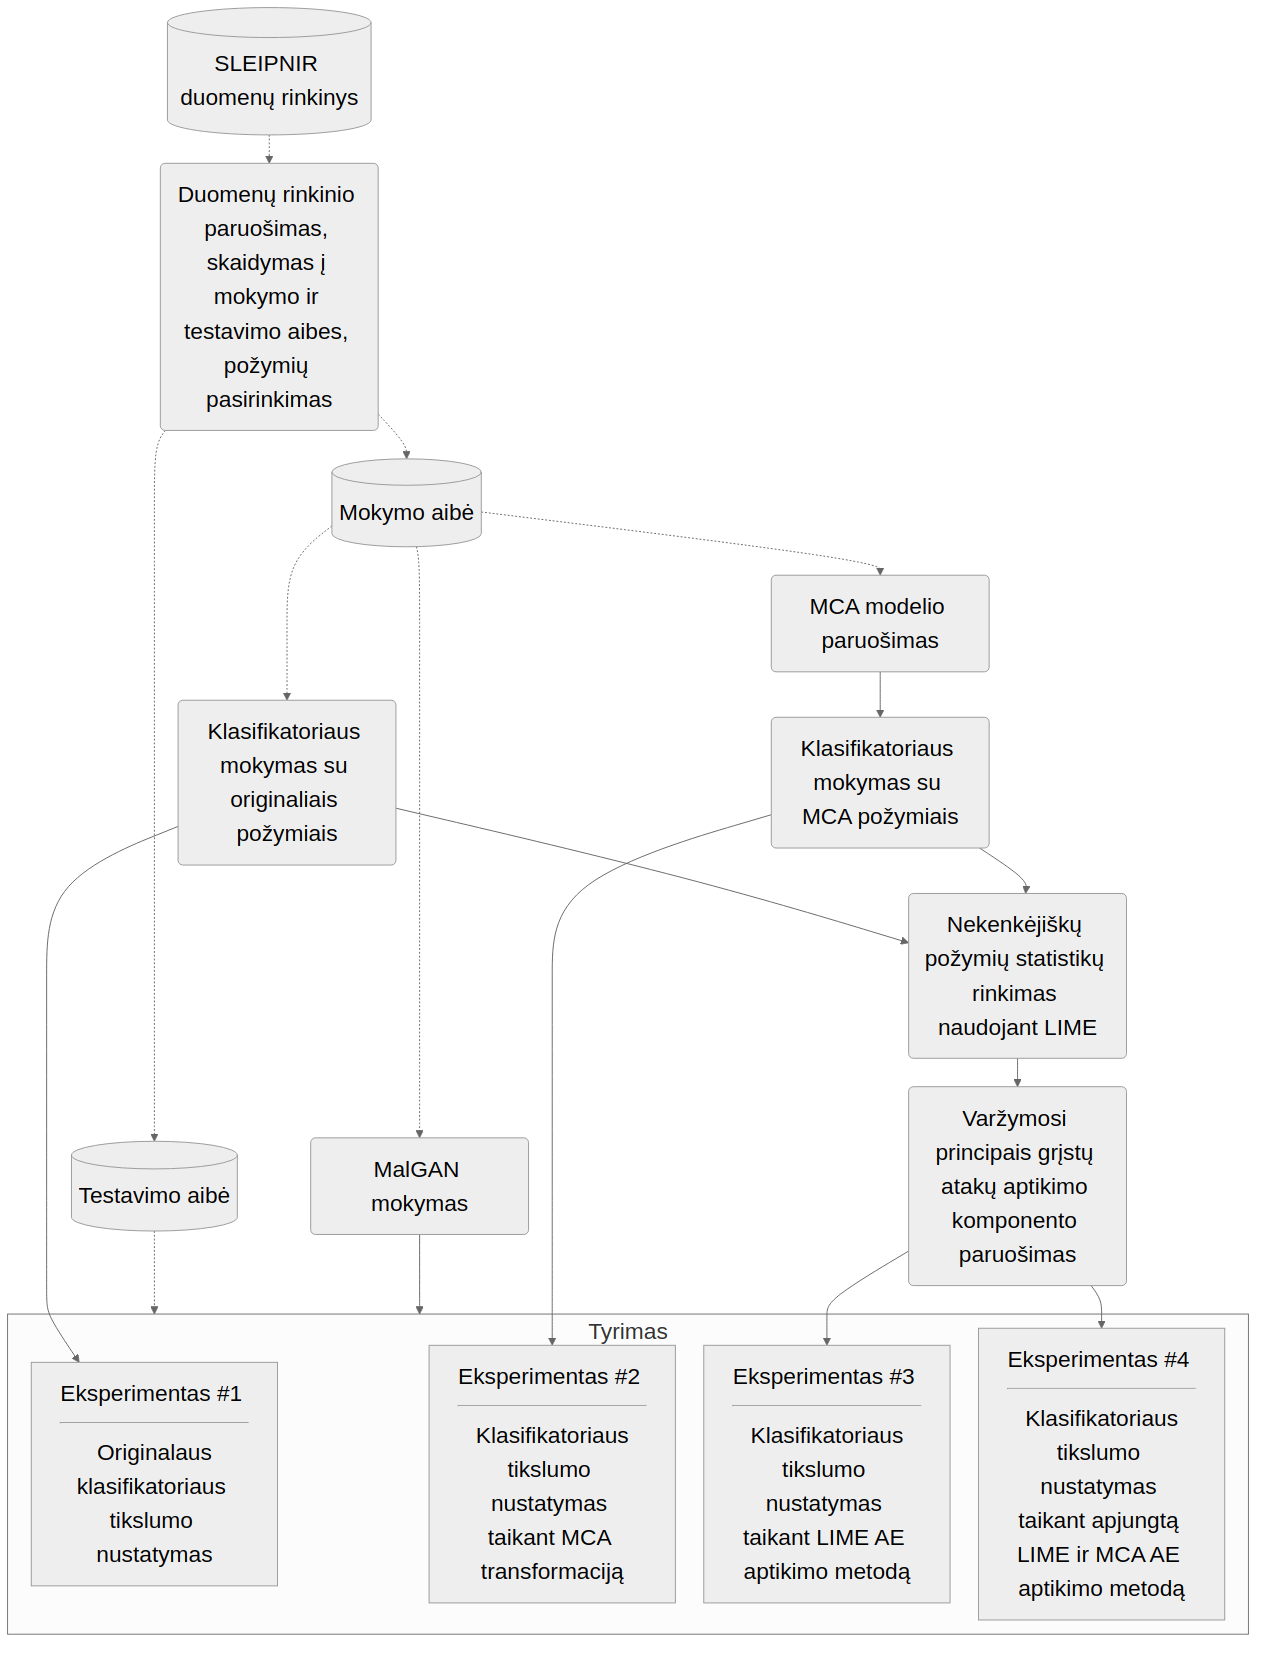
\includegraphics[width=0.95\textwidth]{images/methodology.png}
    \caption{Tyrimo metodika}
    \label{fig:methodology}
\end{figure}

\begin{figure}[h]
    \centering
    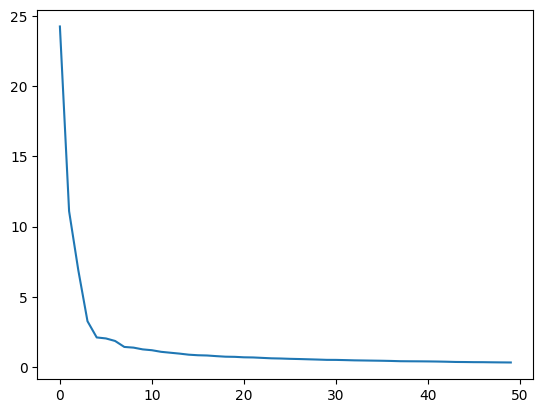
\includegraphics[width=0.45\textwidth]{images/inertia_50.png}
    \caption{\textit{Alkūnės} analizė \gls{mca} inercijai}
    \label{fig:inertia}
\end{figure}

% --- PCA/MCA
% Show graphs of 2 best components (~30% of inertia)
% Show knee analysis of 50 then 9 components